\section{Usability}
\label{sec:usability}

Many news articles were published to announce the release of the Safeplug in addition to a lengthy discussion on the Tor-talk mailing list~\cite{tormailinglist}.  There were many thoughts on the Terms of Service and the option to use the device as a Tor relay node; this inspired us to start our analysis with these items.  

\subsection{Terms of Service}
\label{tos}
The Terms of Service (TOS) contains three main points of interest: TOS updates, open source licensing information, and software updates.

\subsubsection{TOS updates} Pogoplug suggests that users consistently read the TOS becaues they can update or change them at anytime.  Most Safeplug users will likely not read the TOS once, let alone on a regular basis; therefore, most users will be blind to any changes.  It is also interesting that these TOS are only accessible through a small link at the bottom of the Safeplug website \cite{safeplug}; specifically, there is no documentation, including the TOS, in the package that the device was shipped in.

\subsubsection{Open source licensing information}  There is a section that acknowledges the use of many open source components in the Safeplug device; this section includes the statement: 

\begin{quotation}
``You agree to abide by the terms of the relevant licenses, as may be updated by Pogoplug from time to time at http://pogoplug.com/home-en-developers-open-source.html. '' \cite{safeplug}
\end{quotation}

The link included is a dead link and takes the user to a web page with a 404 error.  This lack of attention to detail or respect for open source licenses does not put Pogoplug in a good light.  In fact, the Tor-talk mailing list noted this particularly, since Tor is an open source project \cite{tormailinglist}.

\subsubsection{Software updates} Not only can the TOS be updated at any time, so can the software on the device.  These udpates will be ``automatically delivered'' to the user, but the user is not notified of these updates~\cite{safeplug}.  This should raise a red flag for users because they may not know when the software in their device is being changed or what it is changing to.  While Safeplug makes many claims about providing anonymity, users are simply putting their trust in a different entity, namely Pogoplug.

\subsection{Tor Relay Node Option}
One of Safeplug's configurations is the use of the device as a Tor relay node in the Tor network.  When the device is initially setup, the default setting is to not use it as a relay node.  

One of our concerns is how understandable this setting is to the average Internet user.  The settings page describes Tor in an extremely basic way:

\begin{quotation}
``Safeplug uses the Tor network to secure your Internet connection.  Tor works by routing your Internet through a series of random destinations, much like driving a twisty, complicated route to throw off someone who is following you, making it impossible for websites and organizations to identify the source or destination of Internet traffic.'' \cite{safeplug}
\end{quotation}

On the other hand, it describes the functionality of a Tor relay node in a much more technical manner.  This description is shown in Figure~\ref{fig:relaydesc}.  If the majority of users can only understand the simpler description, then they likely won't understand the description of a Tor relay node.  This could be a problem if users simply decide not to do anything with that setting (i.e. don't change the setting to use Safeplug as a relay node).  Then there would be a large increase in use of the Tor network, yet most of the users are not giving back to it.

\begin{figure}[th]
\begin{center}
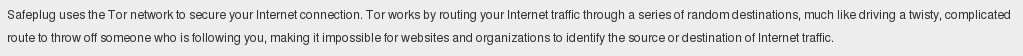
\includegraphics[width=\textwidth]{funnydesc.png}
\caption{Description of Tor on Safeplug settings page.}
\label{fig:funnydesc}
\end{center}
\end{figure}

\begin{figure}[th]
\begin{center}
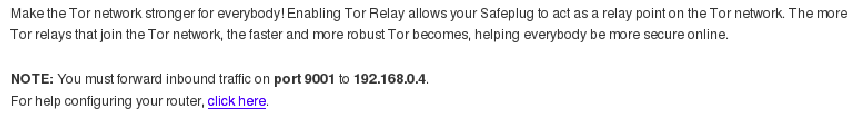
\includegraphics[width=\textwidth]{relaydesc.png}
\caption{Description of a Tor relay on Safeplug settings page.}
\label{fig:relaydesc}
\end{center}
\end{figure}

This could easily be remedied; Safeplug should choose a target audience and have consistent descriptions.  The best option is to explain the Tor network and the functionality of a Tor relay node at the same level, preferably a level that normal Internet users can understand.  This increases the chances that users will run their Safeplug as a relay node.

\subsection{Internet Use}
\label{inetuse}
Figure~\ref{fig:before} shows what a web page looks like before turning Tor and ad-blocking on, while Figure~\ref{fig:after} shows the same website after turning Tor and ad-blocking on.  Both of these figures show our IP address in the top right corner; due to the change in IP address we can see that our traffic is being routed through Tor.  

\begin{figure}[htb]
\centering
\begin{subfigure}[b]{.4\textwidth}
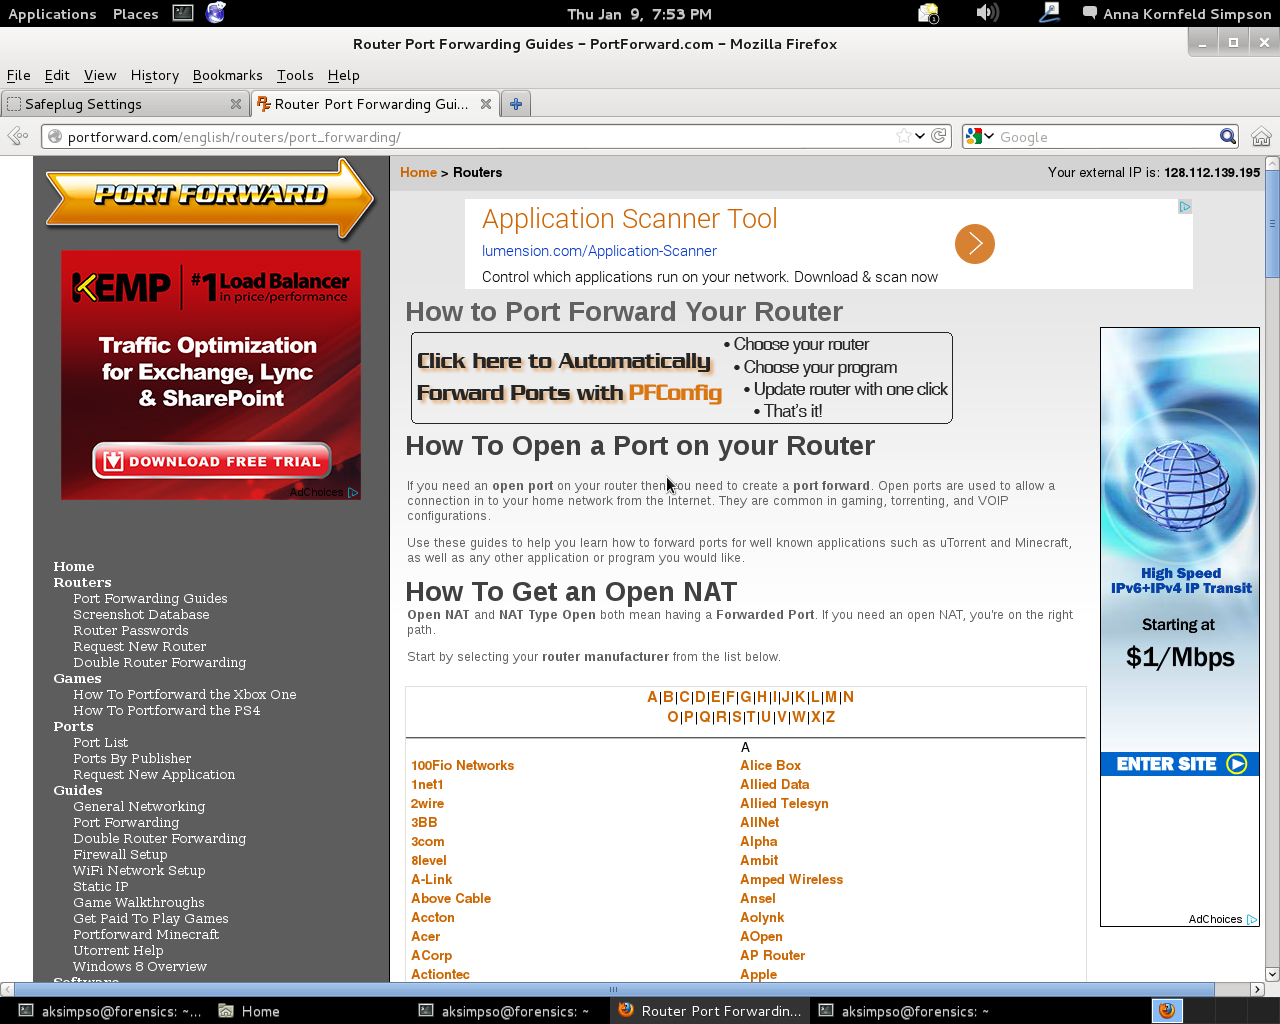
\includegraphics[width=\textwidth]{before}
\caption{Web page before using Tor and ad-blocking.}
\label{fig:before}
\end{subfigure}%
\quad
\begin{subfigure}[b]{.4\textwidth}
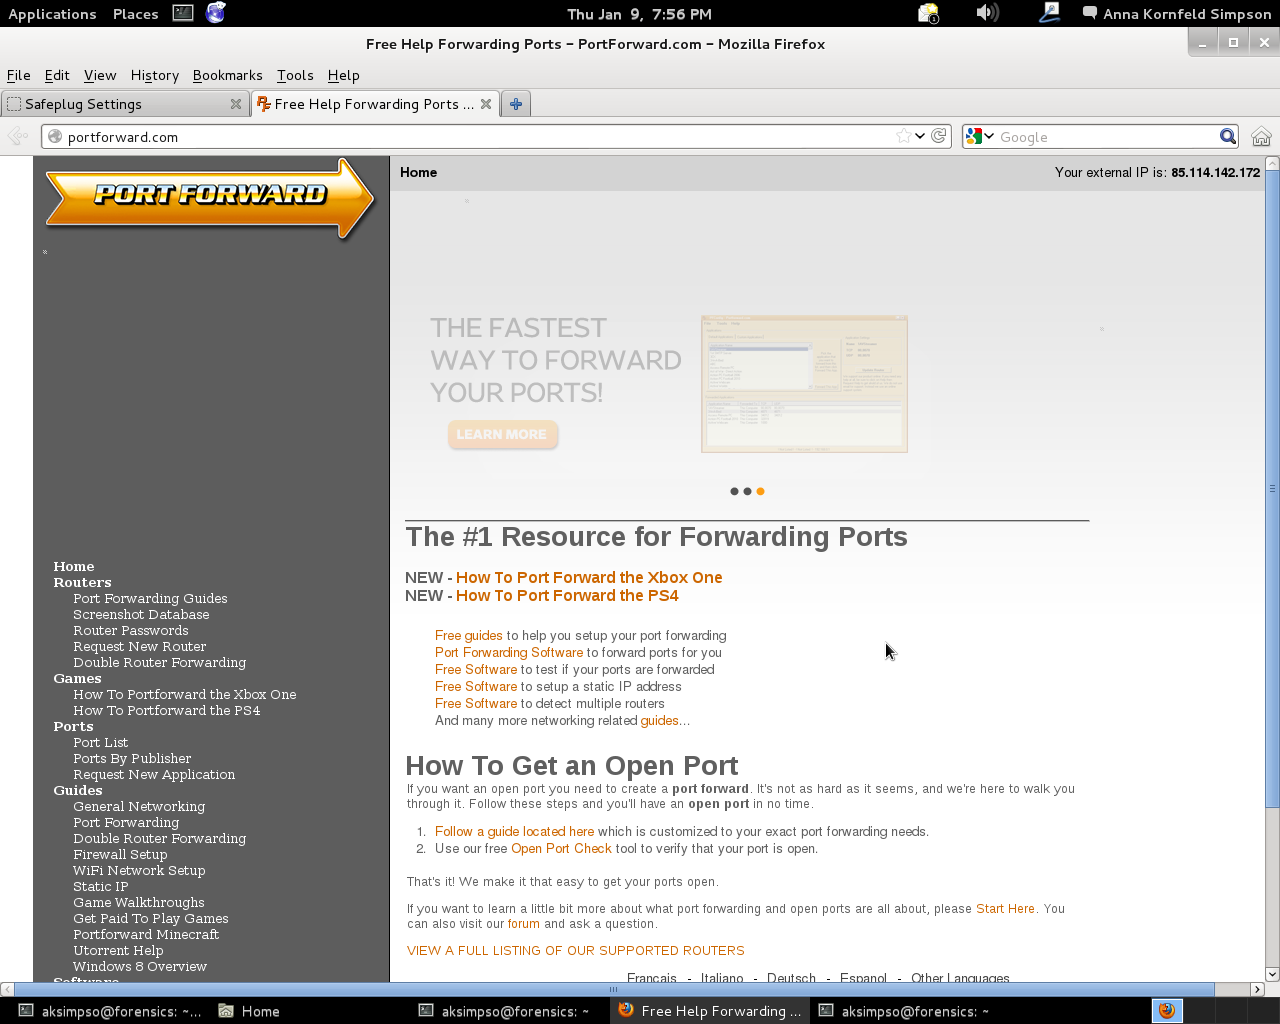
\includegraphics[width=\textwidth]{after}
\caption{Web page after using Tor and ad-blocking.}
\label{fig:after}
\end{subfigure}
\end{figure}

Next, we wanted to see how usable this would be to a normal Internet user.  A user would probably decide not to use Safeplug if they could not read their web pages (if they were not in their native language), or if they could not log into their accounts (some web sites will lock a user out if they try to log in from multiple countries in a short time period).  While browsing the Internet, we experienced some pages in German and Swedish, which is expected with Tor; if a user is not familiar with Tor, then they may just get frustrated and stop using Safeplug altogether.  We were also prompted with the page in Figure~\ref{fig:funnygoogle} when we tried to log into our Google account, indicating that Google noticed we were trying to login from different locations.

\begin{figure}[htb]
\begin{center}
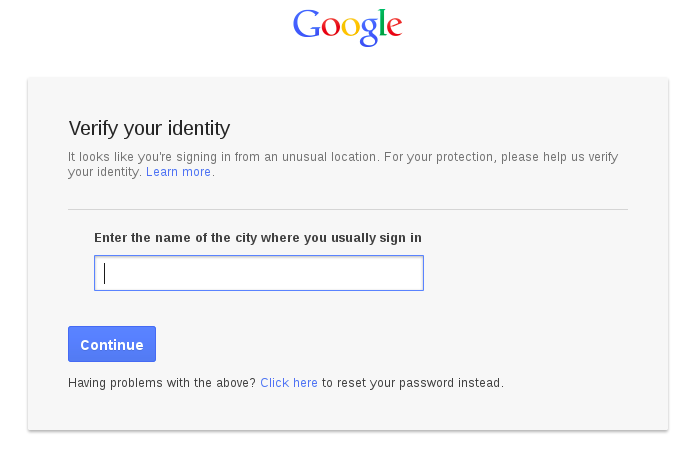
\includegraphics[width=0.5\textwidth]{funnygoogle}
\caption{Google's response after trying to log in.}
\label{fig:funnygoogle}
\end{center}
\end{figure}

\subsection{Cookies}  
While browsing the Internet, we logged into a Google Account in a tab, and then subsequently went to a website that had the Google+ logo in a different tab.  When we clicked on the Google+ logo, it remember who we are; so we can confirm that we still have first-party cookies.  We experienced the same situation with Facebook and its corresponding ``like'' button.

This is clearly not the perfect ``anonymity'' that Safeplug promised in their publicity.  Although normal use does follow this model of persisting logged in status across browser tabs and sessions, a user concerned about anonymity and seeing each session coming up differently (German vs Swedish) might mistakenly believe that they do not have to log out of their social media accounts to preserve their anonymity when accessing other websites.

More interesting and damaging to the user's control over their anonymity would be third-party cookies because the user cannot remove those just by logging out.  It requires a trip to the browser settings to clear cookies (or not have them set in the first place).  We used the FourthParty plugin developed by Jonathan Mayer at Stanford to collect information about cookies and other browsing data during the client's use of the Safeplug \cite{fourthparty}.  When collecting data on the existence of third-party cookies, we analyzed two separate browsing sessions; they were both new sessions with no cookies.  One of the sessions used the ad-block feature of the Safeplug and the other did not.  After analyzing data from Fourthparty, we found many third-party cookies in both sessions.  These included cookies from: abmr.net, bizographics.com, krxd.net, and bluekai.com among many others.

\subsection{Latency}
If the latency of web requests using the Safeplug is noticeably longer than that of normal Internet use, users may be deterred from using the device.  Similarly, if turning Tor on, but not ad-blocking, adds a significant time delay, the user may only turn on the ad-blocking feature (without Tor).  We recorded the time for a web request on the following settings:

\begin{itemize}
\item Plain Firefox
\item Firefox, no Tor, no ad-blocking
\item Firefox, Tor, no ad-blocking
\item Firefox, Tor, ad-blocking
\item Firefox, no Tor, ad-blocking
\item Tor Browser Bundle with Safeplug (all settings turned off)
\item Tor Browser Bundle
\end{itemize}

For each of the settings, we took 20 measurements; Figure~\ref{fig:latency2} shows the average time of a web request on each of the specified settings for three different web pages.  The differences between web pages can most likely be attributed to the amount of ads on the web page.  

\begin{figure}[htb]
\begin{center}
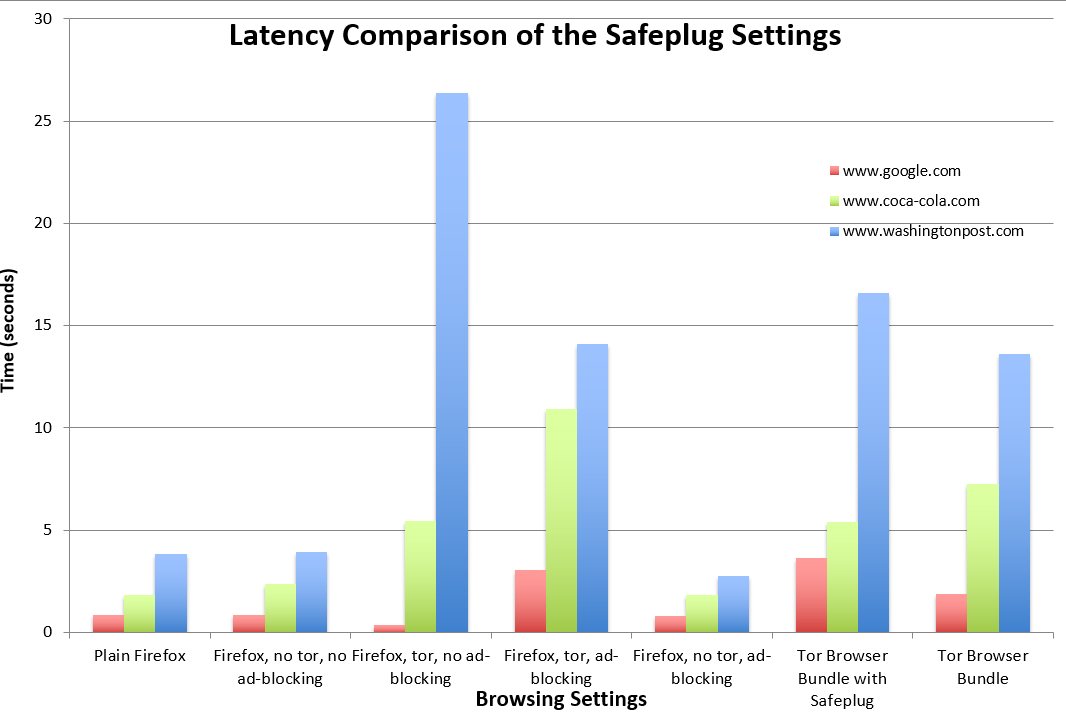
\includegraphics[width=0.7\textwidth]{latency2}
\caption{Latency of web requests.}
\label{fig:latency2}
\end{center}
\end{figure}

It is interesting to note that the average web request time for accessing \url{www.washingtonpost.com} is greatest on the same settings that the average web request time for \url{www.google.com} is the least. This setting did not include ad-blocking, and therefore \url{www.washingtonpost.com} had to render each ad; \url{www.google.com} does not have any ads.  This also explains why the average latency was greater than the other settings for \url{www.washingtonpost.com}: each ad was requested through Tor.   

The latency of using the Safeplug with Firefox, Tor, and ad-blocking is comparable to that of using the Tor Browser Bundle.  For all three web pages, the Tor Browser Bundle had slightly lower latency.  
